%%%%%%%%%%%%%%%%%%%%%%%%%%%%%%%%%%%%%%%%%
% Structured General Purpose Assignment
% LaTeX Template
%
% This template has been downloaded from:
% http://www.latextemplates.com
%
% Original author:
% Ted Pavlic (http://www.tedpavlic.com)
%
% Note:
% The \lipsum[#] commands throughout this template generate dummy text
% to fill the template out. These commands should all be removed when 
% writing assignment content.
%
%%%%%%%%%%%%%%%%%%%%%%%%%%%%%%%%%%%%%%%%%

%----------------------------------------------------------------------------------------
%	PACKAGES AND OTHER DOCUMENT CONFIGURATIONS
%----------------------------------------------------------------------------------------

\documentclass{article}

\usepackage{fancyhdr} % Required for custom headers
\usepackage{lastpage} % Required to determine the last page for the footer
\usepackage{extramarks} % Required for headers and footers
\usepackage{graphicx} % Required to insert images
\usepackage{lipsum} % Used for inserting dummy 'Lorem ipsum' text into the template
\usepackage{enumerate}
\usepackage{booktabs}
\usepackage{amsmath}

% Margins
\topmargin=-0.45in
\evensidemargin=0in
\oddsidemargin=0in
\textwidth=6.5in
\textheight=9.0in
\headsep=0.25in 

\linespread{1.5} % Line spacing

% Set up the header and footer
\pagestyle{fancy}
\lhead{\hmwkAuthorName} % Top left header
\chead{\hmwkClass\ (\hmwkTitle)} % Top center header
%%\rhead{\firstxmark} 
\rhead{} % Top right header
\lfoot{\lastxmark} % Bottom left footer
\cfoot{} % Bottom center footer
\rfoot{Page\ \thepage\ of\ \pageref{LastPage}} % Bottom right footer
\renewcommand\headrulewidth{0.4pt} % Size of the header rule
\renewcommand\footrulewidth{0.4pt} % Size of the footer rule

\setlength\parindent{0pt} % Removes all indentation from paragraphs

%----------------------------------------------------------------------------------------
%	DOCUMENT STRUCTURE COMMANDS
%	Skip this unless you know what you're doing
%----------------------------------------------------------------------------------------

% Header and footer for when a page split occurs within a problem environment
\newcommand{\enterProblemHeader}[1]{
\nobreak\extramarks{#1}{#1 continued on next page\ldots}\nobreak
\nobreak\extramarks{#1 (continued)}{#1 continued on next page\ldots}\nobreak
}

% Header and footer for when a page split occurs between problem environments
\newcommand{\exitProblemHeader}[1]{
\nobreak\extramarks{#1 (continued)}{#1 continued on next page\ldots}\nobreak
\nobreak\extramarks{#1}{}\nobreak
}

\setcounter{secnumdepth}{0} % Removes default section numbers
\newcounter{homeworkProblemCounter} % Creates a counter to keep track of the number of problems

\newcommand{\homeworkProblemName}{}
\newenvironment{homeworkProblem}[1][Problem \arabic{homeworkProblemCounter}]{ % Makes a new environment called homeworkProblem which takes 1 argument (custom name) but the default is "Problem #"
\stepcounter{homeworkProblemCounter} % Increase counter for number of problems
\renewcommand{\homeworkProblemName}{#1} % Assign \homeworkProblemName the name of the problem
\section{\homeworkProblemName} % Make a section in the document with the custom problem count
\enterProblemHeader{\homeworkProblemName} % Header and footer within the environment
}{
\exitProblemHeader{\homeworkProblemName} % Header and footer after the environment
}

\newcommand{\problemAnswer}[1]{ % Defines the problem answer command with the content as the only argument
\noindent\framebox[\columnwidth][c]{\begin{minipage}{0.98\columnwidth}#1\end{minipage}} % Makes the box around the problem answer and puts the content inside
}

\newcommand{\homeworkSectionName}{}
\newenvironment{homeworkSection}[1]{ % New environment for sections within homework problems, takes 1 argument - the name of the section
\renewcommand{\homeworkSectionName}{#1} % Assign \homeworkSectionName to the name of the section from the environment argument
\subsection{\homeworkSectionName} % Make a subsection with the custom name of the subsection
\enterProblemHeader{\homeworkProblemName\ [\homeworkSectionName]} % Header and footer within the environment
}{
\enterProblemHeader{\homeworkProblemName} % Header and footer after the environment
}
   
%----------------------------------------------------------------------------------------
%	NAME AND CLASS SECTION
%----------------------------------------------------------------------------------------

\newcommand{\hmwkTitle}{Problem Set\ \#3} % Assignment title
\newcommand{\hmwkDueDate}{Sunday,\ February\ 18,\ 2018} % Due date
\newcommand{\hmwkClass}{FIN\ 514} % Course/class
\newcommand{\hmwkClassTime}{9:30am} % Class/lecture time
\newcommand{\hmwkAuthorName}{Wanbae Park} % Your name

%----------------------------------------------------------------------------------------
%	TITLE PAGE
%----------------------------------------------------------------------------------------

\title{
\vspace{2in}
\textmd{\textbf{\hmwkClass:\ \hmwkTitle}}\\
\normalsize\vspace{0.1in}\small{Due\ on\ \hmwkDueDate}\\
\vspace{3in}
}

\author{\textbf{\hmwkAuthorName}}
\date{} % Insert date here if you want it to appear below your name

%----------------------------------------------------------------------------------------

\begin{document}

\maketitle

%----------------------------------------------------------------------------------------
%	TABLE OF CONTENTS
%----------------------------------------------------------------------------------------

%\setcounter{tocdepth}{1} % Uncomment this line if you don't want subsections listed in the ToC

%%\newpage
%%\tableofcontents
\newpage

%----------------------------------------------------------------------------------------
%	PROBLEM 1
%----------------------------------------------------------------------------------------

% To have just one problem per page, simply put a \clearpage after each problem

\begin{homeworkProblem}
	 %% Sub-Problem a.
	Using the following Black-Scholes formula, the option price was calculated as 10.2479.
	%% Black-Scholes Formula
%----------------------------------------------------------------------------------------
	\begin{equation*}
	\begin{aligned}
		\text{\textit{Put option price}} &= Ke^{-r(T - t)}N(-d_2) - Se^{-\delta (T - t)}N(-d_1)	\\
		d_1 &= \frac{log(\frac{S}{K}) + (r - \delta + \frac{1}{2} \sigma^2)(T - t)}{\sigma \sqrt{T - t}}	\\
		d_2 &= d_1 - \sigma \sqrt{T - t}
	\end{aligned}
	\end{equation*}
%----------------------------------------------------------------------------------------
	Then, using Cox, Ross and Rubinstein(CRR), Rendleman and Bartter(RB), Leisen and Reimer(LR) method each, put option value was calculated from $N = 50$ to $N = 1000$. Figure \ref{fig:prob1-error} shows the error of each method. The error was calculated using the formula $V_N - V_{EXACT}$.
	%% Error Figure
	\begin{figure}[ht]
		\centering
		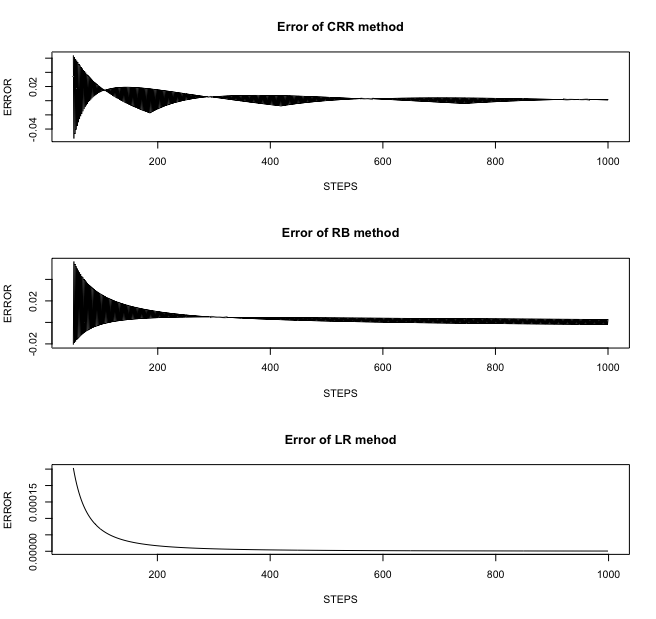
\includegraphics[scale = 0.5]{Q1/error.png}
		\caption{Error of each method}
		\label{fig:prob1-error}
	\end{figure}
	As shown in figure, except LR method, there seems to exist some problems. In CRR method, it looks like that error is converging to zero, but it is not monotonic. It means it does not guarantee that applying more steps makes more accurate values. Regarding RB method, it seems better than CRR, but error is increasing from some points(about $N = 300$). The reason for this phenomenon is that option payoff is not linear shape. Since LR method solves this problem when $N$ is odd, the shape of error in LR method seems monotonically decreasing to zero as $N$ goes to some large value. The reason why monotonicity is important is that we can extrapolate values from two binomial trees to get more accurate values if monotonic error is guaranteed. Figure \ref{fig:prob1-error_extra} shows the error after extrapolation($M = 2N$ is used when using CRR and RB method, $M = 2N - 1$ is used for extrapolation.).
	%% Extrapolation
	\begin{figure}[ht]
		\centering
		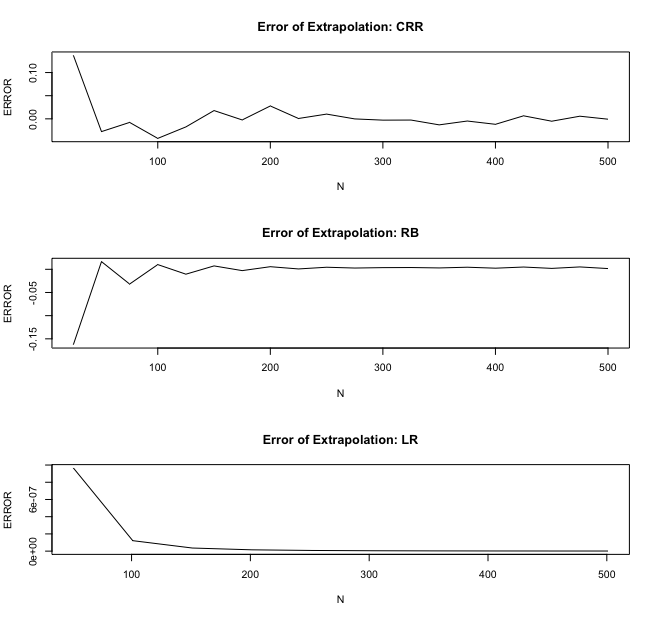
\includegraphics[scale = 0.5]{Q1/errorextra.png}
		\caption{Error of each methods after extrapolation}
		\label{fig:prob1-error_extra}
	\end{figure}
	Since it is well-known that LR method has $O(1/n^2)$ errors, the extrapolation procedure has changed from original one to followings.
	\begin{equation*}
		V_{EXACT} \approx \frac{M^2 V_M - N^2 V_N}{M^2 - N^2} ~~ \text{where $M$ and $N$ are odd numbers.}
	\end{equation*}
	%% Accuracy of extrapolation: CRR, RB(X), LR(O) because of monotonicity
	As shown in Figure \ref{fig:prob1-error_extra}, the error of CRR and RB methods seems sawtoothing, but error of LR method is converging to zero monotonically. Furthermore, the accuracy of value is even worse at some points for CRR and RB method when extrapolation is applied. Before using extrapolation technique, the maximum error of CRR and RB method is about 0.05, but there are some points where error is about 0.1 after extrapolation. However, in LR method, the error after extrapolation is always smaller than before. That is why monotonicity is important when using extrapolation to get more accurate value.
\end{homeworkProblem}

%----------------------------------------------------------------------------------------
%	PROBLEM 2
%----------------------------------------------------------------------------------------
\begin{homeworkProblem}
	The value of American put option is calculated as 10.3762 using Broadie and Detemple(BD) method for 10000 steps. All following procedures are performed assuming this number is true value of the option. Using the same procedure of Problem 1, errors were calculated using CRR, BD, LR method. Figure \ref{fig:prob2-error} shows errors of each method.
	%% Error Figure
	\begin{figure}[ht]
		\centering
		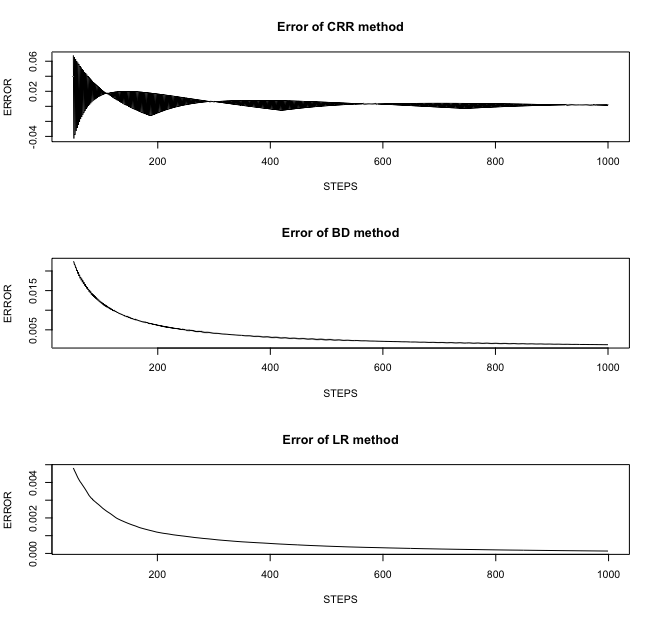
\includegraphics[scale = 0.5]{Q2/error.png}
		\caption{Error of each method}
		\label{fig:prob2-error}
	\end{figure}
	In similar to result of European option, error of CRR method seems to have sawtoothing shape and periodic humps when valuing American options. Moreover, the amount of error is even larger than errors of case in European options. In contrast, the other two methods seems to have errors converging to zero monotonically. Since it is already known that sawtoothing and periodic humps of error comes from non-linearity of payoff, and in European or American option case, the non-linearity occurs only at the maturity of option, error of BD method has monotonicity and convergence because the method avoid pricing option at maturity. LR method also avoid non-linearity using other parameters to construct binomial tree, errors of LR method also have good features. In other words, CRR method has problems because it has no efforts to handle non-linearity problems. The problem of CRR method also occurs when calculating exercise bound of options. Figure \ref{fig:prob2-boundary} shows the exercise boundary using CRR method.(the number 0 of plot means early exercise is not optimal at the step.) 
	%% Exercise boundary of CRR
	\begin{figure}[ht]
		\centering
		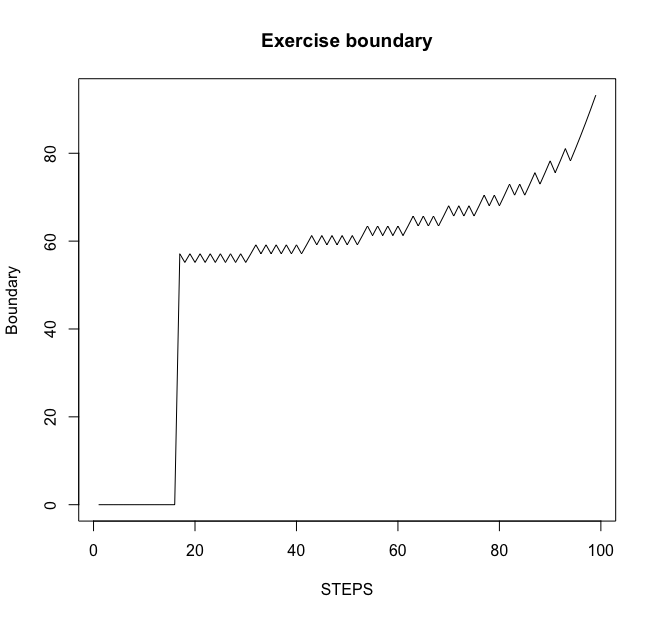
\includegraphics[scale = 0.5]{Q2/boundary.png}
		\caption{Exercise boundary: CRR method}
		\label{fig:prob2-boundary}
	\end{figure}
	Theoretically, the exercise boundary of a put option should be a smooth increasing function. However, as shown in figure, the shape of boundary is sawtoothing, which does not coincide with theory. Since the optimal exercise boundary is distorted under CRR method, exercise-or-not decision at each node will be distorted consequently, and finally it causes distortion of option prices.	\\
	Similar to Problem 1, it is possible to reduce error using extrapolation technique, if monotonically decreasing error is guaranteed. For each method, we calculated errors of option price using extrapolation technique. Figure \ref{fig:prob2-error_extra} shows the error of each method using extrapolation technique.
	%% Extrapolation Error
	\begin{figure}[ht]
		\centering
		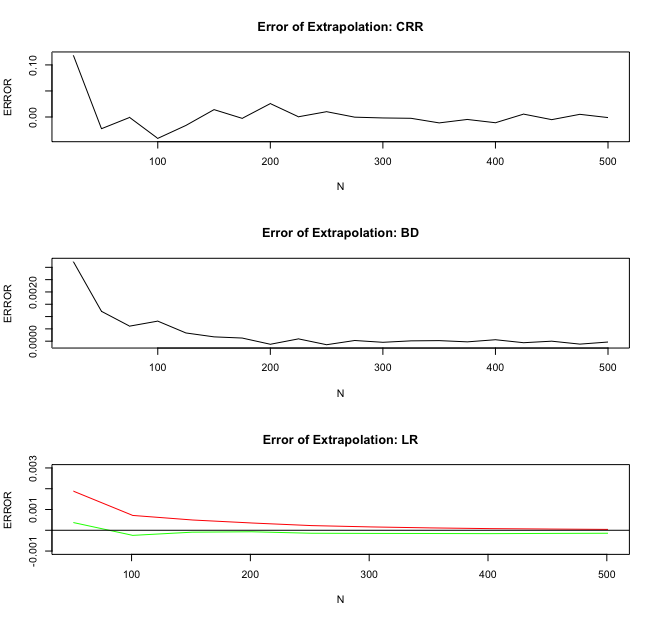
\includegraphics[scale = 0.5]{Q2/errorextra.png}
		\caption{Error of each methods after extrapolation}
		\label{fig:prob2-error_extra}
	\end{figure}
	errors of all three methods seems to converge to zero. However, because of non-monotonicity, errors in CRR methods using extrapolation is larger than errors not using extrapolation technique in some points. The other methods seem to have smaller errors than not using extrapolation because they have monotonic errors. The interesting thing is errors of LR method. In graph of LR method of Figure \ref{fig:prob2-error_extra}, the red line is the value of errors using extrapolation of error of order 2, and the green line is which of order 1. The horizontal black line is \textit{Error} = 0 line. It is easy to expect that extrapolating with order 2 is better than with order 1. Of course, extrapolating with order 2 has faster convergence speed, however, at small $N$, extrapolating with order 1 is more accurate than extrapolating with order 2.
\end{homeworkProblem}

%----------------------------------------------------------------------------------------
%	PROBLEM 3
%----------------------------------------------------------------------------------------
\begin{homeworkProblem}
	Using the analytic formula given in problem set, the analytic price of option is calculated as 5.61756. It will be used for the following procedures. In order to analyze the performance of CRR model, we calculated option prices from $N = 50$ to $N = 1000$ and plotted error. Figure \ref{fig:prob3-error} shows error of CRR method for pricing down-and-out call option.
	%% Error of Barrier Option
	\begin{figure}[ht]
		\centering
		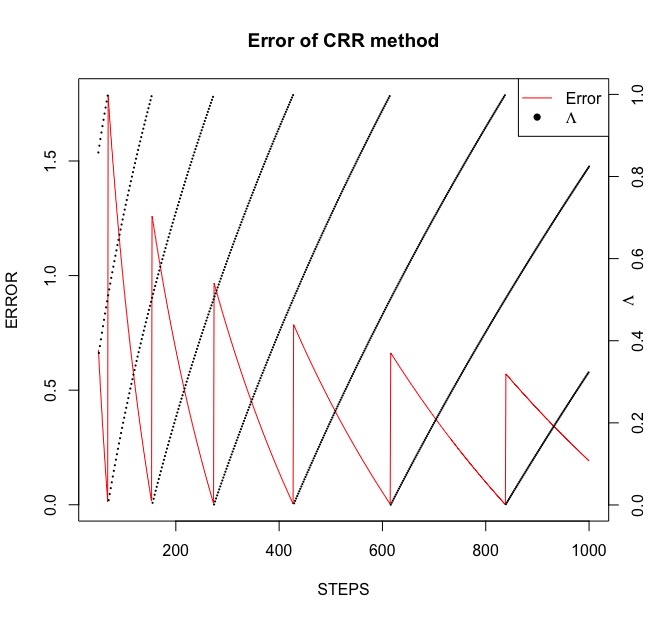
\includegraphics[scale = 0.5]{Q3/error.png}
		\caption{Error of CRR method}
		\label{fig:prob3-error}
	\end{figure}
	In Figure \ref{fig:prob3-error}, errors is much larger than errors of European or American options. Therefore, it needs to be careful when pricing barrier options using CRR model. Moreover, the shape of error is periodic and there is a point where the error increases sharply from zero. After the error increases rapidly from zero, it decreases again to zero. To analyze this feature, we used a measure $\Lambda$, which represents relative position of barrier of nodes. It is calculated as followings.
	\begin{equation*}
	\begin{aligned}
		&\Lambda = \frac{S_k - B}{S_k - S_{k-1}}	\\
		&S_k:~\text{the closest node above the barrier}	\\
		&S_{k-1}:~\text{the node below the barrier}	\\
		&B:~\text{barrier}
	\end{aligned}
	\end{equation*}
	If $B = S_k$, then $\Lambda$ will be equal to zero, and if $B = S_{k - 1}$, then $\Lambda$ will be equal to one. That means $\Lambda$ has a value between zero and one, and if barrier is exactly equal to some value of node, $\Lambda$ will be equal to zero or one. In this figure, we used $\Lambda$ with node at maturity. From the figure, we can observe that error is approximately equal to zero when $\Lambda$ is equal to zero or one. It means that the value of barrier option is calculated accurately if barrier of option is exactly at some value of node. Otherwise, the error would be enormously large even if the barrier is very slightly different to the value of node. %% c.
	Since we know the behavior of error corresponding to $\Lambda$, it is possible to use this property to improve convergence of model. It is observed that error which have equal corresponding $\Lambda$ has monotonically decreasing features as number of steps increases. Therefore, if we choose several steps which makes equal $\Lambda$, and get set of option values, then use extrapolation technique for pricing options, the accuracy would be increased since the errors of the set is monotonically decreasing.
\end{homeworkProblem}

\end{document}